\documentclass{Preport}
\usepackage{ctex}
\usepackage{hyperref}
\usepackage{amsmath, amsthm, amssymb, amsfonts}
\usepackage{esint}
\usepackage{nicematrix}
\usepackage{extarrows}
\usepackage{graphicx}
\usepackage{enumitem}
\usepackage{multirow, booktabs}
\usepackage{caption}
\usepackage{float}
\usepackage[dvipsnames]{xcolor}
\usepackage[english]{babel}
\usepackage{bm}
\usepackage{cite}
\hypersetup{
    colorlinks=true,
}

\exname{光速测量} %实验名称
\instructor{张利} %指导教师
\class{生医2402} %班级
\name{姚舜瑜} %姓名
\stuid{3240100532} %学号

\nyear{2025} %年
\nmonth{9} %月
\nday{23} %日
\nweekday{二} %星期几

\begin{document}
\setcounter{page}{0}
\makecover

\section{预习报告(10分)}
\subsection{实验综述(5分)}
\subsubsection{实验原理}
本实验采用光调制法测量光速。基本原理如下:

假设我们让一个光源照射一个接收器,二者距离为$\Delta S$,我们就可以通过测量光信号到达接收器的时间差$\Delta t$,从而计算出光速$c=\frac{\Delta S}{\Delta t}$。
但由于光速极快,直接测量时间差$\Delta t$非常困难,因此我们采用相位法测量光速。我们使用一个周期性调制的光源发射光信号,其光强为$I=I_0 +\Delta I_0 \cos(2\pi \upsilon t)$。
将其转化为变化的电压信号$U=U_0 \cos(2\pi \upsilon t)$。我们通过测量光信号到达接收器时产生的电压信号与初始信号之间的相位差$\Delta \phi$,从而计算出时间差$\Delta t=\frac{\Delta \phi}{2\pi \upsilon }$,进而计算出光速$c=\frac{2\pi \upsilon  \Delta S}{\Delta \phi}$。

但由于此时,调制频率 $\upsilon $ 的值较大,光程 $\Delta S$ 很小的距离变化都可能引起相位差 $\Delta \phi$ 的急剧变化,用示波器难以精确测量。
因此,我们采用和差频法进行处理。将接收到的含有相位差 $\Delta \phi$ 的高频信号 $U_2 = A_2 \cos(2\pi \upsilon t - \Delta\phi)$ 与另一个频率为 $\upsilon ''$ 的高频信号 $U_3 = A_3 \cos(2\pi \upsilon ''t)$ 进行差频。
根据三角函数积化和差公式,混频后得到的信号为:
\begin{equation}
U_2 \cdot U_3 \propto \cos(2\pi(\upsilon +\upsilon '')t - \Delta\phi) + \cos(2\pi(\upsilon -\upsilon '')t - \Delta\phi)
\end{equation}

该信号包含一个和频分量和一个差频分量(忽略振幅)。
接着,使用一个滤波器滤除高频的和频信号,只保留低频的差频信号 $\upsilon ' = \upsilon  - \upsilon ''$。得到的最终信号为 $U' \propto \cos(2\pi \upsilon 't - \Delta\phi)$。
而处理后的低频信号 $U'$ 与原始高频信号 $U_2$ 具有完全相同的相位差 $\Delta\phi$。
这样,我们就可以通过精确测量容易观察的低频信号的相位差 $\Delta\phi$,来间接测量高频信号的相位差 $\Delta\phi$。

\begin{figure}[H]
    \centering
    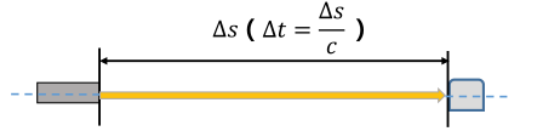
\includegraphics[width=0.6\textwidth]{理论原理图.png}
    \caption{相位法测量光速原理}
    \label{fig:相位法原理}
\end{figure}

在实验真实使用的光速测量仪器上,由于光源和接收器放在一起,光信号是经过反射镜反射后再到达接收器的,因此光程实际上是 $2\Delta S$。
那么高频信号的相位差为 $\Delta\phi = 2\pi \upsilon  \Delta t = 2\pi \upsilon  \frac{2\Delta S}{c}$,而低频信号的相位差为 $\Delta\phi = 2\pi \upsilon ' \Delta t'$,且两者相位差相等,
整理后即可得到最终用于计算光速的公式:

\begin{equation}
\label{eq:光速公式}
c = \frac{2(s_2 - s_1)\upsilon }{\Delta t' \upsilon '}
\end{equation}

其中,$s_2 - s_1$ 是光程差 $\Delta S$,$\upsilon $ 是原始高频频率, $\upsilon '$ 是差频频率,$\Delta t'$ 是在示波器上测得的低频信号时间差。

\begin{figure}[H]
    \centering
    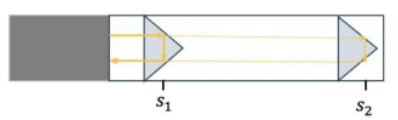
\includegraphics[width=0.4\textwidth]{真实仪器示意图.png}
    \caption{真实仪器示意图}
    \label{fig:真实仪器示意图}
\end{figure}

于是,根据上述理论原理,我们制造出了如下仪器:
\begin{figure}[H]
    \centering
    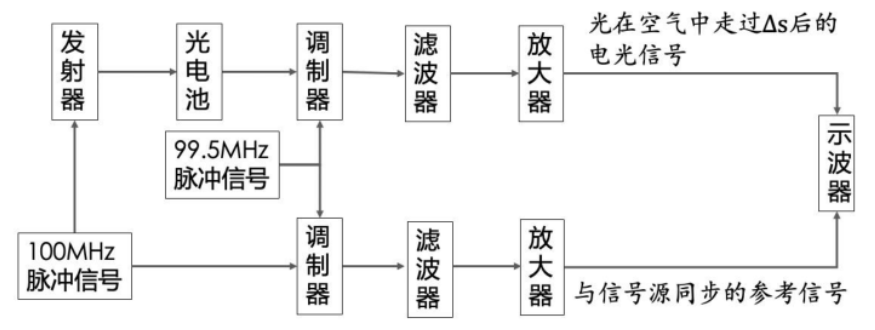
\includegraphics[width=0.8\textwidth]{仪器原理.png}
    \caption{仪器原理}
    \label{fig:仪器原理}
\end{figure}


\subsubsection{实验方法}
本实验主要器材包括:1、光速测量仪;2、示波器;


\textbf{Step 1.} 开启电源,调节光路,确保发射光能准确地反射回接收器中心,以获得最强的信号。

\textbf{Step 2.} 取第一个六等分点为$S_1$,利用示波器$Track$功能将光标1对齐测量信号幅度峰值。保持光标1位置不变。

\textbf{Step 3.} 移动反射镜到剩余的六个等分点$S_2$至$S_6$,每移动到一个点,利用示波器$Track$功能将光标2对齐测量信号幅度峰值,记录此时的时间差$\Delta t'$。

\textbf{Step 4.} 根据测得的六个时间差$\Delta t'$和对应的光程差$s_2 - s_1$,利用公式\eqref{eq:光速公式}计算出光速$c$的值。

\textbf{Step 5.} 略微改变$S_1$的位置,重复上述步骤,获取更多数据,计算平均值并估算误差。




\subsection{实验重点(3分)}
1. 理解相位法测量光速的基本原理和实验方法。

2. 学会通过“逐差法”或“累积法”减小测量误差。

\subsection{实验难点(2分)}
1. 光路调节:精确调节光路,确保发射光能准确地反射回接收器中心,以获得最强的信号。

2. 示波器使用:熟练掌握示波器的各项功能,特别是$Track$功能,以便准确测量信号的时间差。

3. 数据处理:合理处理测量数据,计算光速并估算误差。


\newpage
{\fangsong \noindent \textbf{注意事项:}

\begin{enumerate}[label=\arabic*.]
    \item 用PDF格式上传“预习报告”,文件名:学生姓名+学号+实验名称+周次。
    \item “预习报告”必须递交在“学在浙大”本课程内对应实验项目的“作业”模块内。
    \item “预习报告”还须拷贝到“实验报告”中(以便教师批改)。
    \item “大学物理实验”课程选做实验使用本“预习报告”;必做实验无须写预习报告,前往“学在浙大”完成预习测试即可。
\end{enumerate}}
\begin{center}
    \fbfangsong{浙江大学物理实验教学中心制}
\end{center}
\end{document}
